% !TeX spellcheck = <none>
\documentclass[a4paper, 12pt]{article}  

\usepackage[a4paper, margin=2cm, bmargin=2.5cm, tmargin=2.5cm]{geometry}

\usepackage[ngerman]{babel}
\usepackage[utf8]{inputenc}
\usepackage{tgcursor}

\usepackage{amsmath,amssymb,amstext}
\usepackage{color, colortbl}
\usepackage{tikz}
\usepackage{listings}
\usepackage{graphicx}
\usepackage{scrextend}
\usepackage[linkcolor=black,
			hidelinks]{hyperref}
\usepackage{array}
\usepackage{tcolorbox}
\usepackage{trfsigns}
\setcounter{tocdepth}{3}  
\setlength{\arrayrulewidth}{0.1pt}
\setlength{\parindent}{0pt}

\newcommand{\myGreen}{green!50!black}
\newcommand{\myGray}{black!50}

\begin{document}
	\begin{titlepage}
		\center 
		\textsc{\huge \bfseries Merkzettel, Reminder Sheet}\\[1cm] 
		\textsc{\Large }\\[0.5cm] 
		\textsc{\large Author: Bernd Heufelder}\\[0.5cm] 
		{\large \today}\\[1cm] 
		
\includegraphics[width=0.3\linewidth]{./pics/BesiLogo.jpg}\\[1cm]
		\begin{flushleft}
			\tableofcontents
		\end{flushleft}
	\end{titlepage}
	
	\part{Pragmatisches}
	\section{Verbindungsaufbau mit der Maschine}
	\begin{itemize}
		\item PuttY starten
		\item Maschinenname eingeben, z.B. fc-4438
		\item Benutzername: ses\\
	  Passwort: dmsu
		\item Mushell starten
		\item In der Mushell: Ultimet\_startETNE eingeben um Maschine "freizuschalten"
		\item Im Port-File muss die Maschine definiert sein, dann kann übers Dropdown-Menü die Verbindung/Maschine ausgewählt werden um eine Verbindung herzustellen.
	\end{itemize}
	Beispiele für \textit{port.properties} Einträge verschiedener Maschinen. Die Grünen Einträge sind immer gleich und rot ist variabel.
	\begin{itemize}
		\item \textbf{FlipChip (fc)/8k8}
		\begin{addmargin}[0.2cm]{0cm}
			\begin{tabular}{lp{11cm}}
				port.\textcolor{red}{8}.name=\textcolor{red}{fc-4169} & \textcolor{\myGray}{Beliebiger Name, diser wird im Dropdown Menü angezeigt}\\
				port.\textcolor{red}{8}.driver=\textcolor{red}{etn://fc-4169:1160} & \textcolor{\myGray}{Maschinenname, muss mit der Beschilderung auf der Maschine übereinstimmen}\\
				port.\textcolor{red}{8}.protocol=\textcolor{\myGreen}{ETB}&\\
				port.\textcolor{red}{8}.accept.0.driver=\textcolor{\myGreen}{ETN:0}&\\
				port.\textcolor{red}{8}.start=\textcolor{\myGreen}{auto}&\\
			\end{tabular}
		\end{addmargin}
		\item \textbf{Lupus Testunit}
		\begin{addmargin}[0.2cm]{0cm}
			\begin{tabular}{lp{11cm}}
				port.\textcolor{red}{8}.name=\textcolor{red}{Lupus testunit-401} & \\
				port.\textcolor{red}{8}.driver=\textcolor{red}{etn://testunit-401:1160} &\\
				port.\textcolor{red}{8}.protocol=\textcolor{\myGreen}{ETB}&\\
				port.\textcolor{red}{8}.accept.0.driver=\textcolor{\myGreen}{ETN:0}&\\
				port.\textcolor{red}{8}.start=\textcolor{\myGreen}{auto}&\\
			\end{tabular}
		\end{addmargin}
		\item \textbf{Evo/2k2}
		\begin{addmargin}[0.2cm]{0cm}
			\begin{tabular}{lp{9cm}}
				port.\textcolor{red}{8}.name=\textcolor{red}{EVO 2-modulig evo-005089 } & \textcolor{\myGray}{Beliebiger Name, diser wird im Dropdown Menü angezeigt}\\
				port.\textcolor{red}{8}.driver=\textcolor{red}{etn://evo-005089:1160} & \\
				port.\textcolor{red}{8}.protocol=\textcolor{\myGreen}{ETB}&\\
				port.\textcolor{red}{8}.accept.0.driver=\textcolor{\myGreen}{ETN:0}&\\
				port.\textcolor{red}{8}.start=\textcolor{\myGreen}{auto}&\\
			\end{tabular}
		\end{addmargin}
		\item \textbf{Beliebige Maschine}
		\begin{addmargin}[0.2cm]{0cm}
			\begin{tabular}{lp{9cm}}
				port.\textcolor{red}{8}.name=\textcolor{red}{VCB-02\_ssd} & \textcolor{\myGray}{Als Beispiel die VCB-Maschine}\\
				port.\textcolor{red}{8}.driver=\textcolor{red}{etn://10.10.18.109:1160} & \textcolor{\myGray}{Statt Maschinenname kann auch direkt über die IP-Adresse verbunden werden}\\
				port.\textcolor{red}{8}.protocol=\textcolor{\myGreen}{ETB}&\\
				port.\textcolor{red}{8}.accept.0.driver=\textcolor{\myGreen}{ETN:0}&\\
				port.\textcolor{red}{8}.start=\textcolor{\myGreen}{auto}&\\
			\end{tabular}
		\end{addmargin}
	\end{itemize}
\section{Maschineninbetriebnahme}
	Prinzipiell wird das Phasing aller Achsen durchgeführt. Überprüfung aller Encoder. Können alle Achsen gehomed werden? Die Regelung ist bereits getuned.
\section{ComET Command Prompt}
	\subsection{Hilfreiche Kommandos}
		Rufzeichen $ ! $ für alle Achsen und $ .x $ führt das Kommando nur für die aktuell ausgewählte Achse aus.\\\\
		\begin{tabular}{l|p{14cm}}
			\rowcolor{gray!10!white}
			\textbf{name.x} & als Rückgabewert erhält man die Benennung der Achse mit welchler man gerade verbunden ist \\ \rowcolor{gray!10!white}	
			\textbf{ver.x} & Versionsnummer der gerade gewählten Achse (e.g. 0x316xxxx) -> die ersten 3 Ziffern sind die Versionsnummer und die darauf folgenden kennzeichnen die Revision \\	
		\end{tabular}
	\subsection{Undocumented Parameters}
		\begin{tabular}{l|p{14cm}}
			\rowcolor{gray!10!white}
			\textbf{C9} & MLTI Multiplikator \\ \rowcolor{gray!10!white}	
			\textbf{K260} &  \\	
			\textbf{K261} &  \\	
		\end{tabular}
\section{Maschinenbedienung}
\textbf{Kommandos und Tastenkombinationen\\\\}
\begin{tabular}{l|p{14cm}}
	\rowcolor{gray!10!white}
	\textbf{Strg+Shift+F2} & Run Application (z.b. zum Start vom Indel-INCO-Explorer )\\
	\rowcolor{gray!10!white}
	& \begin{itemize}
		\item \textbf{konquer:} Öffnet File-Explorer des Maschinenpc's
		\begin{itemize}
			\item[+] Motion-Files (Seq., Reg., ...) sind im Pfad \textit{Datacon/share/config/Servotools}
		\end{itemize}	
	\end{itemize}	
\end{tabular}

\section{Servo Tools}
	Erweiterung der Servotool durch Eingabe von \textit{servoToolsDialogExpertMode 2} in der Mushell. Z.B. für den Fall wenn sich Register-Files nicht vom PC auf den Controller updaten lassen, kann dies über die Servotools im Expert-Mode manuell geschehen.\\\\
	
	expertMode -> Force overwrite\\\\
	
	Terminal -> Registerwerte auslesen

\section{Servo-Bundle}
	Ist ein .zip-File, in welchem sich das XML-File, sämtliche benötigte Register-Files, Sequenzen und Firmware-Files befinden. Auf jeder Maschine befindet sich das Gesamte zip-File. Ein Servobundle kann für alle Maschinenplatformen verwendet werden, da sich die besagten Files für alle Maschinen darin befinden. Jedes Servobundle hat ein version\_info.txt, in welchem die Änderungen der einzelnen Versionen gelistet sind.\\\\ Sequenzen müssen kompiliert werden bevor sie auf die Maschine überspielt werden. Um ein Kompilieren auf der Maschine zu umgehen wurde der Offline-Sequence-Compiler entworfen. Damit werden die .txt Files in .eseq Files umgewandelt. Im Servo-Bundle befinden sich nur die kompilierten Versionen der Sequenzen.
	\subsection{XML-File}
		Im XML-File sind für jede einzelne Maschine die Folgenden Zuweisungen für jede Achse definiert
		\begin{itemize}
			\item Auf welchem Controller-Typ hängt die Achse
			\item Welche Controller-ID hat die Achse
			\item Mit welcher Firmware soll die Achse laufen
			\item Welche Sequence läuft für die Achse
			\item Welches Register-File ist der Achse zugewiesen
			\item Welches Homing und Phasing soll die Achse verwenden
		\end{itemize}
	\section{Firmenspezifisch}
	\subsection{Firmenstruktur}
		\subsubsection{Software}
			\paragraph{BIB}
				Softwareabteilung, besthend aus OMA und Betriebssystem für die Maschine (Linux).
				\subparagraph{OMA}\leavevmode\\
					Hardwareabstraktion auf Sofwareebene; Applikation erhält möglichst einheitliche Objekte für unterschiedliche Hardware. Die Applikation verwendet diese Hardware dann entsprechend und programmiert damit einen Prozessablauf. Kommunikation der HW über CAN-Bus und PC. OMA ist nicht echtzeitfähig (z.b. Rückmeldung nach Bewegungsende). Bildverarbeitung ist eigenständig und nicht Teil der OMA. Auch wird durch die OMA die Topologie der Hardware, also welche HW an welchem Knoten hängt, verschleiert. \\\\
					Link zur Doku: \hyperlink{dsf}{https://confluence.besi.com/display/MA/interferometric+systems+RENISHAW}
			\paragraph{Applikation}
				Programiert einen Prozessablauf und seine Bewegungen. Ebenso wird die Benutzeroberfläche auf der Maschine von der Applikation bereitgestellt.
	\subsection{Ansprechpersonen}
		\begin{tabular}{l|p{13cm}}
			\rowcolor{gray!10!white}
			\textbf{Simon Holzknecht} & Chef Software Tester, Ansprechpartner zum Reservieren von Maschinen \\
			\rowcolor{gray!00!white}
			\textbf{Michael Kirchler} & Zuständiger System Engineer für 2k2, Umbauarbeiten bei Evo bzw. akutell vorhandene customized Versionen \\
			\rowcolor{gray!10!white}
			\textbf{Bernd Jandl} & Manager Machine Integration Software\\
			\rowcolor{gray!0!white}
			\textbf{Christian Knoll} & Maschinenplanung - Manager System Engineering 2k2 \\
		\end{tabular}
	
	\newpage
	\part{Projektspezifisch}
	\section{Common Control Platform (CCP)}
	
	\subsection{Hardware}
		\textbf{Indelprodukte}
		\begin{itemize}
			\item \textbf{COP-MAS2:} Das CPU-Board ist die zentrale Kontrolleinheit einer Indel Steuerung. Das CPU-Board koordiniert die Achsen und I/O-Systeme in Echtzeit. Alle Indel CPU-Boards werden mit dem Indel Echtzeitbetriebssystem INOS betrieben, dadurch ist es möglich, die gesamte Maschinenapplikation direkt auf dem CPU-Board zu implementieren. Das INOS Betriebssystem übernimmt die Abstraktion der gesamten Hardware und ermöglicht es damit, die gleiche Applikationssoftware auf beliebigen Indel CPU-Boards auszuführen.
			\item \textbf{SAC:} Endstufe zur Motoransteuerung mit integriertem Netzteil
			\item \textbf{SAM4:} High-End Alternative zum COP-MAS mit einer möglichen closed-loop frequenz bis $ 64kHz $.
		\end{itemize}
		\textbf{Besi-Produkte:}
		\begin{itemize}
			\item \textbf{Hammer S3 mit Connection-Board:} Äquivalente Endstufe zum SAC von ESEC selbstentwickelt.
			\item \textbf{UCB: } Notfalleinheit falls COP-MAS ausfällt übernimmt das UCB-Board die Steuerung
		\end{itemize}
		\begin{figure}[!h]
			\centering
			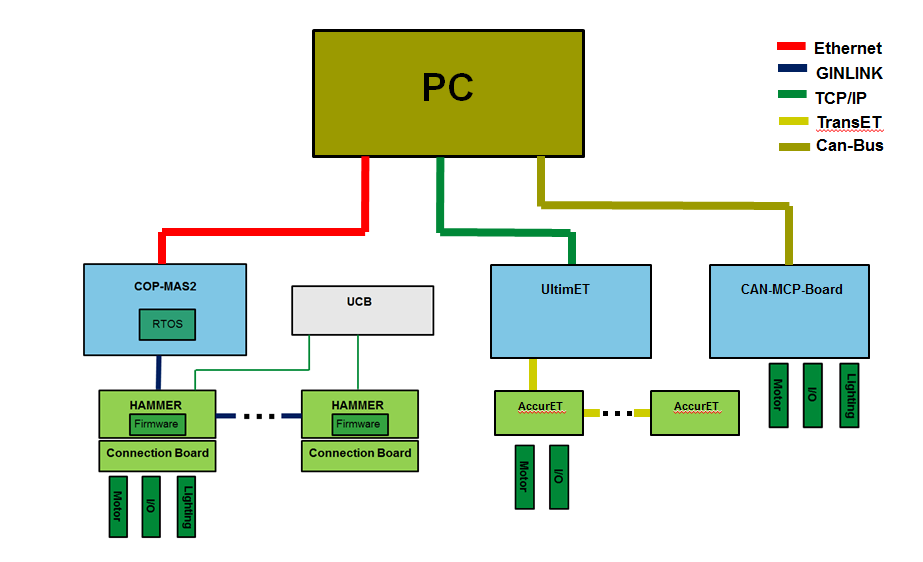
\includegraphics[width=0.85\linewidth]{./pics/ccp/mixed_struktur.png}
			\caption{Gemischte Struktur aus Indel und ETEL Controller}
		\end{figure}
	
		\subsubsection{Kompatibilität Hammer und Connection-Board}
			Beim Starten werden die ID`s der Hammer-Firmware und die ID des Connection-Boards (CB) verglichen. Die ID des CB's ist im Flashspeicher auf dem Board gespeichert. Das Board T128 benötigt dazu die Firmware N128 auf dem Hammer. 
			\begin{figure}[h!]
				\centering
				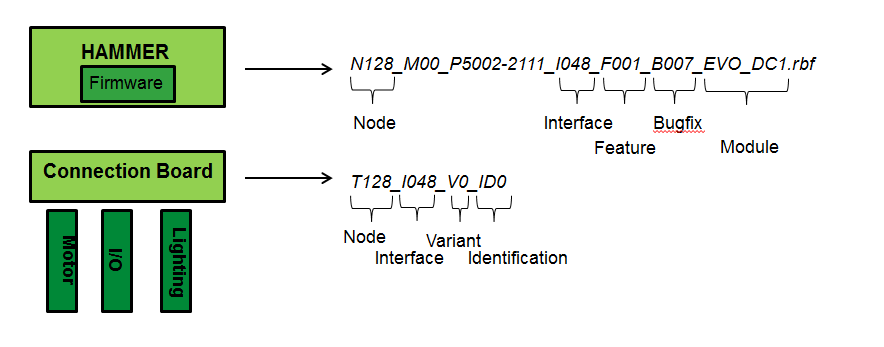
\includegraphics[width=0.8\linewidth]{./pics/ccp/connectionboard.png}
				\caption{ID Übereinstimmung}
			\end{figure}
			Die Identification und Variant kann über Dip-Switches am CB geändert werden. 
		
	\subsection{Konfiguration}
		Die Konfiguration eines Hammer-Boards geschieht anhand von zwei \textit{.dt2} Files, die auf dem MaschinenPC liegen.
		
		Im Source-Code ist der Pfad zu diesen Files hinterlegt. Diese \textit{.dt2} Files sind von Indel und werden direkt vom COP-MAS gelsen.
		\\\\
		Um den Konfigurationsaufwand zu erleichtern werden die Beiden \textit{.dt2} Files von Besi aus mehreren \textit{.dtx} Files erzeugt. Es wird also ein neues Front-End geschaffen, das handlicher zu ändern sein wird.
		
	\subsection{File-Schlacht}
		\subsubsection{\_Objects}
			Dieses File wird automatisch von der Software erstellt, deshalb kann es nicht so einfach ins AxisDefinition integriert werden.
			\begin{figure}[!h]
				\centering
				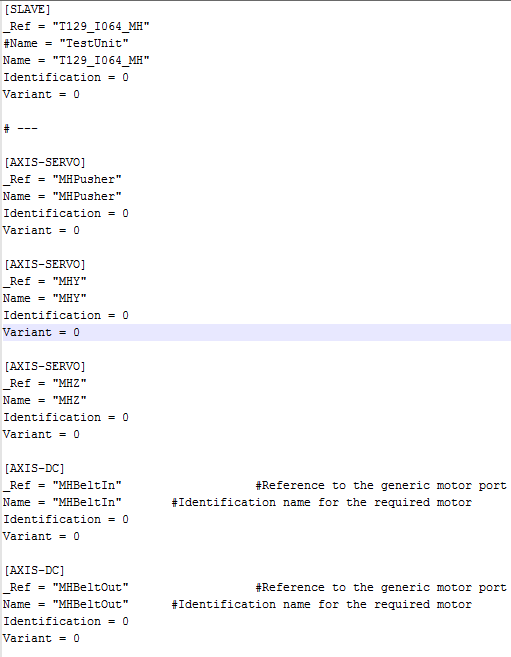
\includegraphics[width=0.8\linewidth]{./pics/ccp/_objects.png}
				\caption{}
				\label{}
			\end{figure}
		\subsubsection{AxisDefinition}
			Hier wird z.b. beim MHPusher auf des Registerfile und die Speedsets dieser Achse verwiesen. Diesen liegen im Subfolder \textit{./Axis}.
			\begin{figure}[!h]
				\centering
				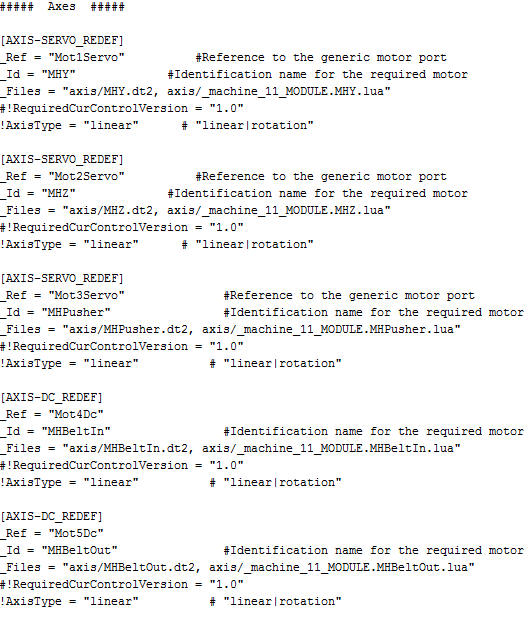
\includegraphics[width=0.9\linewidth]{./pics/ccp/axisdefinition.png}
				\caption{}
				\label{}
			\end{figure}
		\subsubsection{ObjectsDefinitions}
			Es gibt 3 verschiedene Typen an ObjetsDefinition-files:
			\begin{itemize}
				\item ObjectsDefinitions
				\item ObjectsDefinitions-MotX-DC
				\item ObjectsDefinitions-MotX-Servo
				\item ObjectsDefinitions-MotX-Stepper
			\end{itemize}
			In den MotX-Files sind die auf den Motor bezogenen INPUT und OUTPUT Bits den jeweiligen Variablen zugeordnet, wie sie im IO\_Sheet hinterlegt sind. Im \textit{ObjectsDefinitions} sind die Bits für sonstige IO-Signale definiert.
			\begin{figure}[!h]
				\centering
				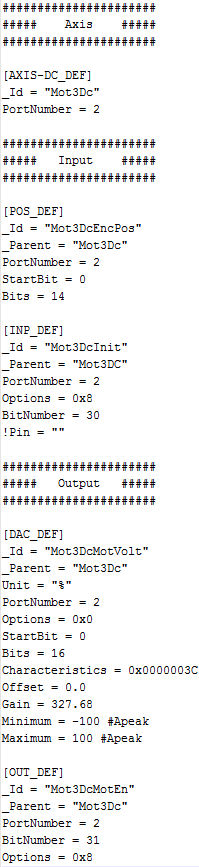
\includegraphics[width=0.3\linewidth]{./pics/ccp/objectsDefinitionServo.png}
				\caption{}
				\label{}
			\end{figure}


	
	
	\newpage
	\part{Theorie}
	\section{Encoder}
	\subsection{SinCos-Encoder}
		Im Abtastkopf leuchtet eine Infrarot-LED seitlich auf eine Maßverkörperung mit reflektierenden und nicht-reflektierenden Bereichen. Das Licht wird von den reflektierenden Bereichen durch ein transparentes Phasengitter zurückreflektiert.
		
		In der Erkennungsebene des Abtastkopfes entstehen hierdurch sinusförmige Interferenzstreifen. Das optische System integriert aus mehreren Teilungsperioden einen Durchschnittswert und filtert Signale heraus, die nicht von der Maßverkörperung reflektiert werden. Dadurch wird die Stabilität des Signals auch dann gewährleistet, wenn die Maßverkörperung verschmutzt oder leicht beschädigt ist.
		
		Durch die einzigartige Optikkonstruktion des Abtastkopfes sowie die Funktionen Auto Gain Control (AGC) und Auto Offset Control (AOC) des REF Interface sind geringe Kurzzeitfehler gewährleistet, die typischerweise einen zyklischen Fehler (SDE) von weniger als +/-0,05 um ergeben.
		
		Das REF Interface verfügt über eine Einstell-LED, die durch ein grünes Licht das Erreichen der optimalen Einstellung anzeigt.
		
		Eine Referenzmarke oder ein einfacher Endschalter sind bei diesem Abtastkopf erhältlich. Die Referenzmarke dient als Referenz oder Nullpunkt für den Abtastkopf, während der Endschalter das Ende des Verfahrbereiches signalisiert.
		\begin{figure}
			\centering
			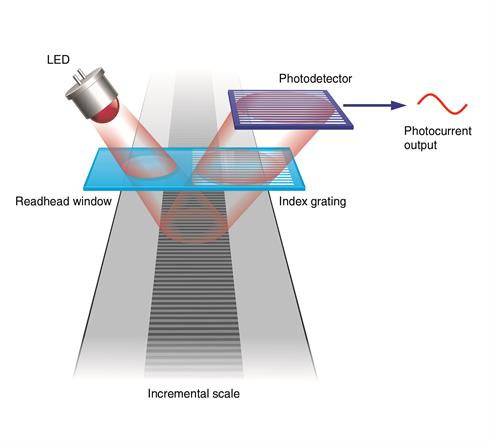
\includegraphics[width=0.7\linewidth]{./pics/sincos_encoder}
			\caption{SinCos Encoder Hardwareaufbau des Encoderkopfs mit Lineal. Das Index Grating ist nur eine transparente Platte.}
		\end{figure}
	\subsection{EnDat Encoder}
		Es gibt ein grobes Lineal in welchem die absolute Position kodiert ist und ein feineres für die inkrementalen Schritte (feinschritt). Die Digitalisierung des Positionswertes erfolgt oft direkt am Encoderkopf.
		\begin{figure}
			\centering
			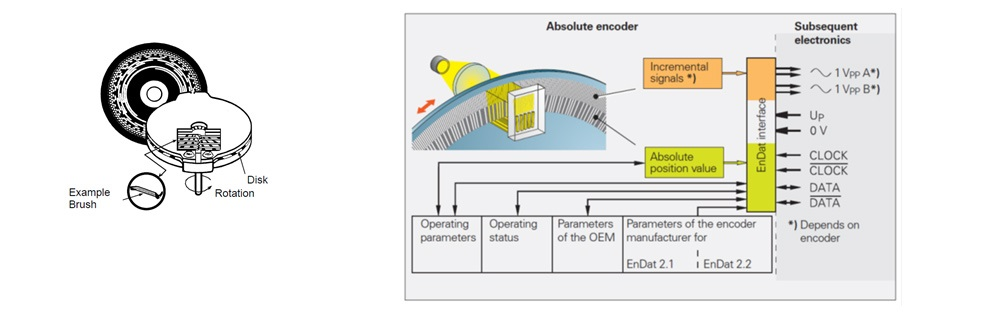
\includegraphics[width=\linewidth]{./pics/endat}
			\caption{Absolutencoder}
		\end{figure}
\section{Bussysteme}
	\subsection{EtherCAT}
		EtherCAT (Ethernet for Control Automation Technology) ist ein von der Firma \textbf{Beckhoff Automation} initiiertes Echtzeit-Ethernet.\\\\
		EtherCAT unterscheidet sich wesentlich von anderen Industrial Ethernet Lösungen. Während bei diesen der vom Master versendete Standard Ethernet Frame (gemäß IEEE 802.3) in jeder Anschaltung zunächst empfangen, dann interpretiert und die Prozessdaten weiterkopiert werden, entnehmen beim EtherCAT die EtherCAT Slave-Geräte die für sie bestimmten Daten, während das Telegramm das Gerät durchläuft. Ebenso werden Eingangsdaten im Durchlauf in das Telegramm eingefügt.\\\\
		Zykluszeiten $ \leq 100 \mu s $ mit niedrigem Jitter.
	\subsection{ETEL Systeme}
		\subsubsection{TransnET}
			Für Echtzeit-Anwendungen mit mehreren Achsen. Die TransnET Synchronisation mit Jitter im Nanosekunden-Bereich ist die richtige Lösung für deterministische und zuverlässige Kommunikation innerhalb von Maschinen.
		\subsubsection{Turbo-ETEL-Bus}
			Multi-axis fast bus mit 100Mbps
	\subsection{CAN-Bus}
		Der CAN-Bus (Controller Area Network) ist ein serielles Bussystem und gehört zu den Feldbussen. Feldbus ist ein Bussystem zur Kommunikation für Sensoren, Aktoren in einer Anlage bzw. Maschine.\\\\
		\textbf{Funktionsprinzip}: Der CAN-Bus arbeitet nach dem „Multi-Master-Prinzip“ d. h., er verbindet mehrere gleichberechtigte Steuergeräte. Ein CSMA/CR-Verfahren löst Kollisionen (gleichzeitiger Buszugriff) auf, ohne dass die gewinnende, höher priorisierte Nachricht beschädigt wird. Der CAN-Bus ist nicht echtzeitfähig, da nicht garantiert werden kann ob der Bus zu gegebenen Zeitpunkt gerade frei ist.
	\subsection{Ginlink}
		Busverbindung vom COPMAS zum Hammer.
\end{document}